A suggested use case for the Data Discovery Library, is to have it run continuously, and analyse the files
live.

The main problem with this use case is that the different analysis functions are expensive to run,
especially when the library tries to build relationships across files.

Therefore, it would be desirable to only run these functions, when it is certain that a file has changed.

The checksum functions however, are not enough in themselves.
Suppose that the library continuously calculated the checksums of the various files:
\begin{enumerate}
    \item It would be extremely slow.
    \item It would be slow to detect changes (e.g. the file changes between the iterations)
    \item If not implemented in a separate thread, it would hang the whole library execution.
\end{enumerate}

The proposed solution is to create a separate program, a file monitor daemon, that runs independently
of the main Data Discovery Library.

There are a few benefits of daemonizing this feature.
Of course the main one, is that it does not affect the performance
of the Discovery Library in any way.
Moreover, if the library crashes for any reason, the files continue to be monitored,
therefore the expensive process of calculating the checksums of all files doesn't have to be repeated.

\subsection{Leveraging Inotify to Reduce the Number of Checksum Calculations}
As mention earlier, it is not realistic to continuously calculate the checksums of all files.

Linux provides a useful API for these situations, inotify ~\cite{Inotify} (other platforms have similar tools available).
It allows one to put monitors on file system objects, whenever a monitored object changes, inotify updates its
file descriptor, from which an application can receive the new events.

The daemon could leverage this API, and only calculate the checksum for files which were flagged by inotify.
A natural question that arises here, is what is the point of calculating the checksum of a file,
if it was already detected as modified by inotify.

However, the API only listens to various system calls, such as \textit{write(2)} or \textit{truncate(2)}.
A simple example, why this is not sufficient to confidently detect changes would be \textbf{echo "" > test.csv}

This simple bash command, would trigger an inotify event, but would not actually change the checksum of the file.

\subsection{Communication Between the Daemon and the Library}
Since the daemon will run as a separate process on the system, some form of interprocess communication (IPC) method
must be utilized.
For this project Unix Domain sockets were chosen due to their simplicity.

\begin{figure}[h]
    \centering
    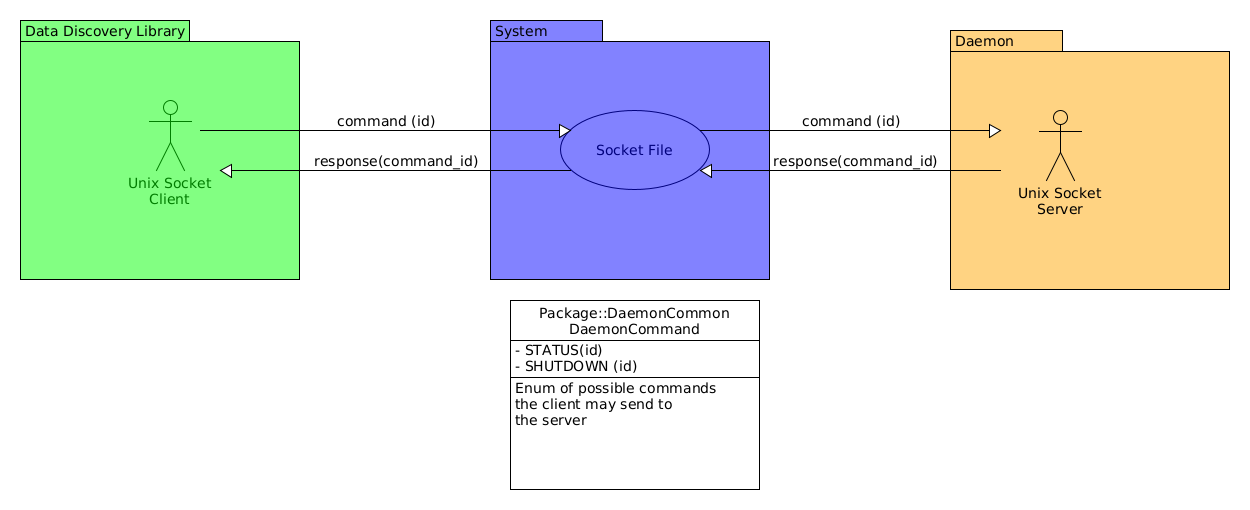
\includegraphics[width=12cm]{figures/daemon/socket_communication}
    \caption{Socket communication between server and client.}
    \label{fig:daemon_fig_1}
\end{figure}


The implementation, essentially needs two components, a socket client (which is part of the Data Discovery Library),
and a socket server, which is part of the daemon.
Their communication is presented on ~\ref{fig:daemon_fig_1}.

The shutdown command, as the name suggests, instructs the daemon to shut down.
It must be called explicitly, as the daemon runs as an independent process, therefore,
terminating the library process, does not implicitly terminate the daemon.

\begin{figure}[h]
    \centering
    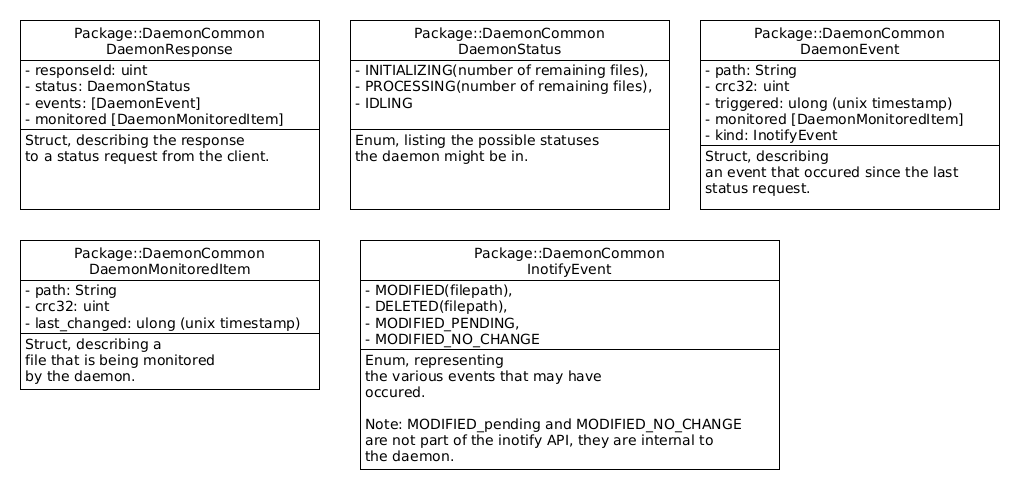
\includegraphics[width=12cm]{figures/daemon/daemon_response}
    \caption{Status response, and accompanying structures.}
    \label{fig:daemon_fig_2}
\end{figure}


The status command invokes the daemon to return the current state of the daemon ~\ref{fig:daemon_fig_2}, alongside the events occurred since the
last status invocation (the event list gets cleared after each status request).
